\documentclass[11pt,a4paper]{article}
\usepackage[T1]{fontenc}
\usepackage[utf8]{inputenc}
\usepackage{lmodern}
\usepackage[margin=1in]{geometry}
\usepackage{amsmath,amssymb,amsthm,mathtools}
\usepackage{booktabs,tabularx,array,longtable}
\usepackage{graphicx,tikz}
\usetikzlibrary{arrows.meta,positioning}
\usepackage{microtype}
\usepackage{enumitem}
\usepackage[round,authoryear]{natbib}
\usepackage[hidelinks]{hyperref}
\usepackage{url}
\setlength{\emergencystretch}{2em}
\setlist{itemsep=3pt,topsep=5pt}
\newtheorem{definition}{Definition}[section]
\newtheorem{theorem}[definition]{Theorem}
\newtheorem{proposition}[definition]{Proposition}
\theoremstyle{remark}
\newtheorem{example}[definition]{Example}
\newcommand{\Pow}{\mathcal P}
\newcommand{\Known}{\mathsf{Known}}
\newcommand{\Unknown}{\mathsf{Unknown}}
\newcommand{\Found}{\mathsf{Found}}
\newcommand{\Conditional}{\mathsf{Conditional}}
\newcommand{\Infeasible}{\mathsf{InfeasibleWithinBound}}
\newcommand{\Req}{\mathsf{Req}}
\newcommand{\Occ}{C_{\mathrm{occ}}}
\newcommand{\All}{C_{\mathrm{all}}}
\newcommand{\status}[1]{\textsf{\small #1}}
\title{MCS: A Formal Framework for Mathematical Knowledge\\
and Learning Routes with External Learner Models}
\author{Peiheng Liu\\\small\href{mailto:peihengmath@gmail.com}{peihengmath@gmail.com}}
\date{October 1, 2026}
\hypersetup{
  pdftitle={MCS: A Formal Framework for Mathematical Knowledge and Learning Routes with External Learner Models},
  pdfauthor={Peiheng Liu},
  pdfsubject={Specification and finite verification of mathematical knowledge and learning routes},
  pdfkeywords={mathematical knowledge representation, learning routes, resource preservation, bounded planning, finite verification}
}
\begin{document}
\maketitle
\begin{abstract}
Relations in mathematical learning resources may encode joint requirements,
alternative entries, proof dependencies, or presentation choices. These meanings
must remain distinguishable when a learner model selects a route or a view hides
part of its context. We present MCS, a specification separating versioned public
mathematical resources, external learner models, and derived views and event
routes. Resource ports retain evidence kind, theory, assumptions, version, and
provenance. We prove a conditional saturation result for concept occurrence
aggregated over unrestricted equivalent expressions; distinguish route-relative
requirements from alternative sufficient supports; and give a compositional
resource-preservation theorem and a bounded exhaustive-search guarantee.
A lossless encoding into an annotated incidence graph makes the representational
boundary explicit. A standard-library Python artifact replays local mathematical
certificates, finite comparison experiments, and a limit-based route example.
On the tested fragment, typed action graphs, annotated bipartite graphs, and MCS
give identical classifications. The contribution is a precise, auditable
integration of interfaces and their guarantees; the results establish neither
unique graph expressiveness nor empirical learning benefits. General correctness
of the Python proof checker and complete machine certification of the mathematical
case studies remain open.
\end{abstract}

\section{Introduction}\label{sec:intro}
A mathematical explanation rarely starts and ends with a node and an arrow.
A proof can require two results together; a definition can be approached
through two representations; and a learner can revisit the same concept in two
different events. Moreover, reading a theorem, obtaining its proof, and being
able to apply it are distinct outcomes. A planning system should say which one
it has produced.

Two motivations lead to the present specification. Within mathematics, an
inference needs the appropriate theory, open assumptions, and evidence, even
when intermediate material is hidden in a compact view. In learning support,
different people need different entry points and may leave some prerequisites
unconfirmed. Their personal records should not silently alter the shared
mathematical content. The first motivation concerns the legitimacy of a resource
connection; the second concerns the ownership and interpretation of a decision.

Consider two actions producing a goal \(g\):
\[
 a_1:\{u,v\}\longrightarrow\{g\},
 \qquad a_2:\{w\}\longrightarrow\{g\}.
\]
If every incoming node edge is treated as required, all of \(u,v,w\) are demanded.
If every edge is treated as sufficient, \(u\) alone appears enough. Explicit
action vertices and grouped input ports resolve this ambiguity.
They do not by themselves resolve another one: an output describing \(g\) is
not necessarily a proof of \(g\). Types, assumptions, versions, and sources must
also be matched. Annotated graph models can retain this information.

The construction develops from entries and links, through grouped actions and
explicit event sources, to a separation of public resources and personal
evaluation. MCS denotes this integrated specification, rather than a new logic
or a psychological law. It supports implementations whose output states both
what a route supplies and why the route was accepted.

\paragraph{Contributions and their status.}
The paper makes three connected contributions.
\begin{enumerate}
\item It specifies a resource and event interface that keeps mathematical
evidence, displayed content, and external learner availability separate.
The principal guarantee is compositional resource preservation under explicit
local validity and source-matching hypotheses
(Theorem~\ref{thm:preservation}).
\item It collects the mathematical boundaries needed by that interface:
unrestricted equivalence can destroy the discriminatory value of concept
occurrence (Theorem~\ref{thm:saturation}); common requirements do not represent
alternative sufficiency; and exhaustive planning is relatively complete only
over an explicitly enumerable finite domain
(Theorem~\ref{thm:search}).
\item It supplies a portable finite artifact, a running mathematical example,
and an equal-information comparison. A constructive incidence-graph encoding
and the finite results identify where no representation advantage
has been established (Proposition~\ref{prop:encoding}).
\end{enumerate}
Several ingredients are elementary applications of established mathematics.
Topological sorting, intersection antitonicity, read-only invariance, and
exhaustive enumeration are not presented as new general theorems. The proposed
contribution lies in their explicit integration with evidence and scope
obligations. No claim of priority for the individual counterexamples is made.

\paragraph{Evidence vocabulary.}
\status{DEF} denotes a definition or modeling choice; \status{PROOF} an argument
given here; \status{REF} an attributed external result or design;
\status{FINITE} an executed check on a stated finite domain;
\status{ILLUSTRATION} stipulated example data; and \status{NOT-CLAIMED} a result
not established here. These labels answer different questions and are not a
ranking of confidence. A passed program run is not a proof that the program is
correct on every input.

\begin{figure}[t]
\centering
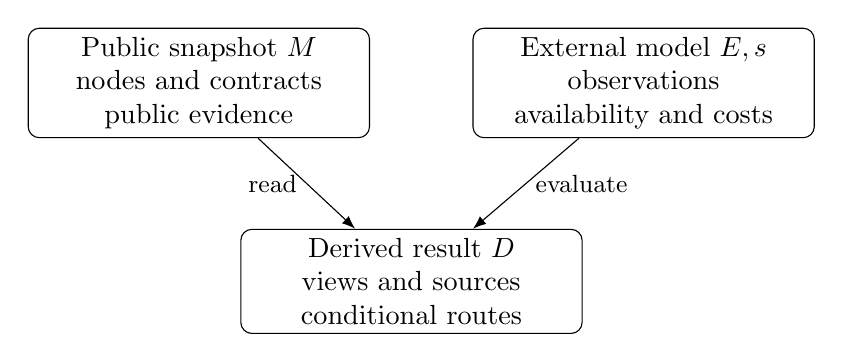
\begin{tikzpicture}[box/.style={draw,rounded corners,align=center,text width=4.1cm,
 minimum height=1.1cm},>=Latex]
\node[box] (m) {Public snapshot \(M\)\\nodes and contracts\\public evidence};
\node[box,right=1.3cm of m] (e) {External model \(E,s\)\\observations\\availability and costs};
\node[box,below=1.15cm of m,xshift=2.7cm] (d)
 {Derived result \(D\)\\views and sources\\conditional routes};
\draw[->] (m) -- node[left,font=\small]{read} (d);
\draw[->] (e) -- node[right,font=\small]{evaluate} (d);
\end{tikzpicture}
\caption{A dependency and ownership contract. Public revision is a separate,
explicit operation. The diagram is a specification, not evidence of an
implementation's isolation or a learner model's validity.}
\label{fig:layers}
\end{figure}

\section{Related work and intended scope}\label{sec:related}
\paragraph{Mathematical knowledge representation.}
OMDoc represents mathematical material at document, statement, and theory
levels \citep{omdoc}. MMT provides a modular representation of theories and
theory morphisms while separating foundation-dependent and
foundation-independent concerns \citep{mmt}. These are direct points of
comparison. MCS resource payloads and evidence can in principle refer to such
libraries. This paper specifies the interface from public resources to
condition-bearing learning events; it does not implement an OMDoc/MMT
translation or prove a stronger representation theorem than those systems.
An MMT \emph{view} is a theory morphism, whereas a view in
Section~\ref{sec:views} is a display projection with a boundary.

\paragraph{Knowledge and learning spaces.}
\citet{spaces} distinguish knowledge spaces from the quasi-ordinal spaces that
are additionally closed under intersection; their Definition~9 and Theorem~10
relate the latter to quasi-orders. We use this existing distinction to situate
the small alternative-entry example in Section~\ref{sec:requirements}.
MCS does not assume that every learner follows a union-closed state family,
that learning is irreversible, or that mathematical nodes coincide with
assessment items. Such assumptions belong to a particular external model.

\paragraph{Partial-order planning.}
The POCL formulation described by \citet{vhpop} includes action instances, causal
links supplying conditions, and ordering constraints; it permits multiple
instances of one action schema. Our event identities and source references have
clear counterparts there. Public resources in the present core are persistent
and reusable: there are no delete effects, so the usual threat problem for
consumed or negated conditions is outside this core. Forgetting and limited
capacity belong to the external schedule predicate. The exhaustive procedure
below is a reference specification, not a competitive POCL planner.

\paragraph{Adaptive educational systems.}
\citet{brusilovsky} describes systems combining domain models, student models,
learning material, and adaptive teaching operations. Separating public content
from student information therefore is not in itself a new architecture.
Here the focus is the status of resources passed between actions,
the scope of a prerequisite assertion, and the conditions under which a
display transformation preserves a route certificate. We do not infer
educational effectiveness from the existence of these interfaces.

\paragraph{The comparison question.}
The relevant question is whether an implementation detects an invalid evidence
connection, preserves unresolved conditions, and reconstructs its decision.
Calling a data structure a graph or a space does not settle that question.
We compare encodings with equivalent annotations and retain negative and equal
results. Formal interoperability with the above systems,
maintenance benefits at scale, and classroom outcomes require further work.

\section{A running example: two approaches to a limit}\label{sec:example}
Let \(D\subseteq\mathbb R\), let \(a\) be an accumulation point of \(D\), and let
\(f:D\to\mathbb R\). There are two familiar ways to state \(f(x)\to L\) as
\(x\to a\): a punctured-neighborhood condition and a condition on every
approaching sequence. A learner comfortable with inequalities may first
inspect the former; a learner familiar with sequences may first inspect the
latter. These are presentation choices, not two different truths.

\begin{definition}[The two statements; \status{DEF}]\label{def:limits}
Write \(\mathrm{ED}(f,a,L)\) for
\[
 \forall\varepsilon>0\ \exists\delta>0\ \forall x\in D:
 0<|x-a|<\delta\ \Longrightarrow\ |f(x)-L|<\varepsilon.
\]
Write \(\mathrm{SEQ}(f,a,L)\) for the assertion that every sequence
\((x_n)_{n\geq1}\) in \(D\setminus\{a\}\) with \(x_n\to a\) satisfies
\(f(x_n)\to L\).
\end{definition}
The puncture excludes the value at the center; the universal quantifier over
sequences prevents one favorable sequence from certifying the limit.
The accumulation-point condition ensures the usual nonvacuous setting and
uniqueness. It is not needed solely for the equivalence below:
at an isolated point both punctured formulations are vacuous.

\begin{proposition}[The limit bridge; \status{PROOF}]\label{prop:limit}
In the stated real metric setting and ZFC metatheory,
\(\mathrm{ED}(f,a,L)\) holds if and only if \(\mathrm{SEQ}(f,a,L)\) holds.
\end{proposition}
\begin{proof}
The forward direction applies one neighborhood bound to a sequence tail.
The reverse constructs a bad sequence if neighborhood control fails.
Assume \(\mathrm{ED}\), and fix an admissible sequence and \(\varepsilon>0\).
Choose \(\delta>0\) as in the definition. Eventually \(|x_n-a|<\delta\);
since \(x_n\neq a\), eventually \(|f(x_n)-L|<\varepsilon\).
Conversely, failure of \(\mathrm{ED}\) gives \(\varepsilon_0>0\) such that
for every \(\delta>0\) there is an \(x\in D\) with
\(0<|x-a|<\delta\) and \(|f(x)-L|\geq\varepsilon_0\).
For \(n\geq1\), choose such an \(x_n\) with \(\delta=1/n\).
This countable choice is available in the stated metatheory.
Then \(x_n\to a\), but \(f(x_n)\not\to L\), a contradiction.
\end{proof}
For continuity assume additionally \(a\in D\). Continuity at \(a\) implies
the punctured condition with \(L=f(a)\). Conversely that condition handles
\(x\neq a\), and the missing case \(x=a\) has zero error.
This proves the continuity bridge in this setting.

It is easy to erase a condition while preserving a plausible picture.
Checking just positive sequences at zero would accept a function equal to
\(1\) on positive reals and \(-1\) on negative reals as having limit \(1\).
Allowing sequences that repeatedly equal the center tests its value too:
if \(f(0)=1\) and \(f(x)=0\) for \(x\neq0\), the punctured limit is \(0\),
but the constant zero sequence does not have image limit \(0\).

The public library records both definitions and the written bridge proof.
A presentation of the bridge statement has a different evidence kind
from the reviewed proof, and both differ from a machine-checked proof object.
The reference route example has four registered actions
(Table~\ref{tab:actions}). The label reviewed records the level of evidence;
it does not assert that external peer review has occurred.

\begin{table}[t]
\centering\small
\begin{tabularx}{\linewidth}{@{}lXX@{}}
\toprule Action & Joint inputs & Output and evidence \\\midrule
\texttt{define\_ed} & Metric, Quantifiers & LimitED content; definition presentation\\
\texttt{define\_seq} & Metric, Sequences & LimitSeq content; definition presentation\\
\texttt{bridge} & LimitED, LimitSeq & Bridge reviewed-proof; Proposition~\ref{prop:limit}\\
\texttt{show\_bridge} & None & Bridge content; statement presentation only\\
\bottomrule
\end{tabularx}
\caption{The executable presentation/reviewed-proof fragment. All ports retain
an explicit real-analysis context. The bridge action records the written proof
as a trust input; it does not mechanically derive it.}
\label{tab:actions}
\end{table}

\begin{figure}[t]
\centering
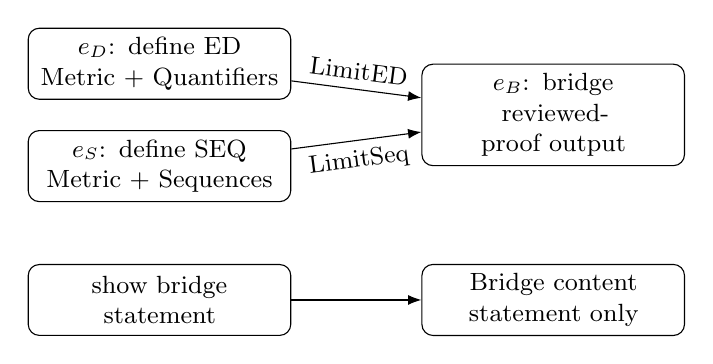
\begin{tikzpicture}[>=Latex,box/.style={draw,rounded corners,align=center,
 text width=3.1cm,minimum height=.9cm},font=\small]
\node[box] (ed) at (0,1) {\(e_D\): define ED\\Metric + Quantifiers};
\node[box] (sq) at (0,-.3) {\(e_S\): define SEQ\\Metric + Sequences};
\node[box] (br) at (5,.35) {\(e_B\): bridge\\reviewed-proof output};
\draw[->] (ed) -- node[above,sloped]{LimitED} (br);
\draw[->] (sq) -- node[below,sloped]{LimitSeq} (br);
\node[box] (show) at (0,-2) {show bridge statement};
\node[box] (content) at (5,-2) {Bridge content\\statement only};
\draw[->] (show) -- (content);
\end{tikzpicture}
\caption{The running case has joint inputs to the bridge event, with either
definition presented first. Showing the same statement separately produces
content, which cannot fill the reviewed-proof target.}
\label{fig:events}
\end{figure}

\section{Public resources and external evaluation}\label{sec:interface}
\subsection{A small public interface}
We work in ordinary set theory. Records and certificates used by an
implementation have finite descriptions; the general public library need not
be finite. The route results require a resource-checking interface rather than
a particular complete logical calculus.

\begin{definition}[Resource descriptor; \status{DEF}]\label{def:resource}
A resource descriptor is a tuple
\[
 r=(n,v,\theta,\kappa,\Delta),
\]
where \(n\) is a node identifier, \(v\) its payload version, \(\theta\) a theory
or context identifier, \(\kappa\) an evidence kind, and \(\Delta\) a declared
finite set of open conditions. A source occurrence is a descriptor together
with a provenance reference. The strict interface matches descriptors by equality.
\end{definition}
Examples of \(\kappa\) are content, declared-assumption, reviewed-proof, and
checked-proof. Equality of node identifiers alone is insufficient.
Conditions are not discharged merely because a source is available.
A checked proof under \(\Delta\) remains conditional on \(\Delta\). A learner's
belief is an external observation, not a proof-resource kind.

Strict matching rejects some legitimate transports, including weakening to a
larger assumption context or moving through a theory translation. Such
transports can be explicit actions with their own evidence.
We do not silently make them part of node equality.

\begin{definition}[Public snapshot; \status{DEF}]
A public snapshot \(M\) contains immutable versioned node payloads, their
representations, a resource registry, public evidence records, and a family
\(\Lambda_M\) of action contracts. Identifiers resolve within a declared
version boundary. Public revision produces a new snapshot or an explicit
version map and is separate from personal-state updates.
\end{definition}
This is the part of the larger MCS organization needed here. Topics,
complete template catalogs, and specialized views can be layered on top.
They are not additional hypotheses of the route theorems.

\begin{definition}[Action contract; \status{DEF}]\label{def:action}
A contract \(a\in\Lambda_M\) consists of a finite indexed input family \(I_a\),
a finite indexed output family \(O_a\), a mode, and local evidence \(w_a\).
Indexed ports allow equal descriptors to have distinct declared roles.
The local validity judgment \(\operatorname{Valid}_M(a,w_a)\) is specified by
the mode and is independent of the existence of a route.
\end{definition}
For a proof-producing action, local evidence accounts for the stated
theory, conclusion, and open conditions. For a presentation action it
accounts for supplied content and its reference. In the finite case study
a written proof is an explicit trusted input. Only the separately replayed
certificate fragment is labeled checked-proof.

\paragraph{Logical boundary.}
A checker may accept a certificate \(p\) for \(T;\Gamma\vdash\varphi\).
Acceptance establishes that judgment only relative to correctness of its
checking rules and their implementation. Truth in a model additionally
requires soundness and satisfaction of \(T,\Gamma\). The main route theorem
is parameterized by local validity and does not prove soundness of a Python
HOL implementation. It makes no completeness claim for standard higher-order
semantics.

\subsection{What is external}
\begin{definition}[External model and result; \status{DEF}]
An external model \(E\) declares a state space \(X_E\), a binding to the public
version, observation and transition interfaces, and a schedule-evaluation
predicate or procedure. A state \(s\in X_E\), goal \(g\), budget \(b\), and
policy \(\rho\) are explicit inputs. A derived result
\[
 D(M,E,s,g,b,\rho)
\]
contains views, candidate event routes, evaluation results, and provenance.
It does not implicitly update \(M\).
\end{definition}
General misconception patterns and assessment items may be public. Who
exhibited a misconception or answered an item belongs to \(E\). A goal separates
its public resource target from a capability claim evaluated by \(E\).
One correct answer need not establish every capability attached to a node.

Unknown information is explicit:
\[
 \operatorname{Info}(A)=\{\Unknown\}\ \sqcup\
 \{\Known(a):a\in A\}.
\]
For supports, \(\Known(\varnothing)\) means a precisely known empty set;
\(\Unknown\) means the support has not been established. For learner input,
unknown availability is neither confirmed availability nor confirmed
unavailability. Missing answers are not stored as wrong answers.

\begin{proposition}[Read-only invariance; \status{PROOF}]\label{prop:readonly}
If every operation used to compute \(D\) reads a fixed snapshot \(M\) and writes
only external or derived records, changing \(E,s,g,b,\rho\) leaves the snapshot
and its registered public relations unchanged.
\end{proposition}
\begin{proof}
Each operation preserves the public record by the write restriction;
induction on any finite execution gives the result.
\end{proof}
The premise is an implementation obligation. Placing personal data
in another table does not establish it. Nor does the proposition compare
truth in two different mathematical models of a theory.

\section{Concept occurrence, support, and alternative requirements}
\label{sec:requirements}
\subsection{A failure of unrestricted equivalence aggregation}
An expression can mention an idea without depending on it. Fix a simply typed
language with lambda abstraction and application. A registry \(K\) assigns each
concept \(c\) a closed typed representation \(t_c\). Let \(\kappa\) map
alpha-normalized closed-term codes to finite sets of registered concepts,
with \(c\in\kappa(t_c)\). This is a naming convention, not a semantic
concept-discovery algorithm.

\begin{definition}[Occurrence and equivalence aggregation; \status{DEF}]
For a finite typed expression \(e\), inspect its unreduced syntax tree.
At each position close the subterm over its free variables in a fixed
context order and apply \(\kappa\). Let \(\Occ(e)\) be the union of these
finite registry answers. For initial representations \(\operatorname{Rep}_0(n)\),
define
\[
 \All(n)=\bigcup_{e_0\in\operatorname{Rep}_0(n)}
                 \ \bigcup_{e\equiv e_0}\Occ(e),
\]
where equivalence keeps the same language, type, theory, and open context.
\end{definition}

\begin{theorem}[Conditional saturation; \status{PROOF}]\label{thm:saturation}
Suppose \(\operatorname{Rep}_0(n)\neq\varnothing\), equivalence contains
ordinary beta-conversion, and occurrence scans the unreduced syntax.
Then \(\All(n)=K\).
\end{theorem}
\begin{proof}
Mention any concept in an unused argument while preserving the expression's
value. Fix \(e_0:\tau\) and \(c\in K\), with \(t_c:\beta\).
For fresh \(z:\beta\),
\[
 e_c=(\lambda z^\beta.e_0)t_c \equiv e_0.
\]
The closed subterm \(t_c\) occurs before reduction, so \(c\in\Occ(e_c)\).
Thus \(K\subseteq\All(n)\). The reverse inclusion follows from the registry's
codomain.
\end{proof}
This concerns the specified function, not all semantic dependency analyses.
With no initial representation the union is empty. If transformations are
only identities, or occurrence is computed after beta-normalization, this
argument fails: a closed constant \(d\) need not mention a distinct registered
constant \(c\). Unnamed semantic objects are outside the registry and theorem.
The result does not recover all concepts from all mathematical meanings.

\subsection{Supports record a use}
Replace the unrestricted union by an indexed family. A support index specifies
a representation or proof or route, its purpose, context, version, and witness.
The support records what that particular object uses, not global necessity.
A proof may contain a redundant premise, and two valid proofs may use
different lemmas. For a fixed purpose \(u\), let
\[
 \mathcal A_u(n)=\{A:\exists w\ \operatorname{Verify}_u(n,A,w)\},
\]
\[
 \operatorname{MinSupp}_u(n)=
 \{A\in\mathcal A_u(n):\nexists B\in\mathcal A_u(n),\,B\subsetneq A\}.
\]
The witness relation must be independently defined. Helping someone understand
is an external empirical predicate, not an unqualified instance of this
public relation.

\begin{proposition}[Minimal supports; \status{PROOF}]
If \(\mathcal A_u(n)\) contains a finite member, it contains an
inclusion-minimal member. If the candidate domain is finite and adequacy is
decidable, all minimal supports can be enumerated.
\end{proposition}
\begin{proof}
Among adequate subsets of one finite adequate set choose one of minimum
cardinality. An adequate proper subset would contradict that choice.
For computation enumerate all candidate subsets and remove each
one containing an adequate proper subset.
\end{proof}
Minimality need not be unique: the sufficient supports \(\{a\}\) and \(\{b\}\)
give alternatives. Infinite adequacy families need not have minimal members;
the cofinite subsets of \(\mathbb N\) are an example.
Inclusion-minimality and minimum cardinality are different objectives.

\paragraph{Safe unknown support.}
Interpret \(\Unknown\) as all subsets of \(K\), and \(\Known(A)\)
as the single possibility \(A\). A set operation returns a precise result only
if all possible inputs give that result. Hence
\(\Unknown\cap\Known(\varnothing)=\Known(\varnothing)\), but in general
\(\Unknown\cap\Known(\{c\})=\Unknown\).
Bounds \(L\subseteq A\subseteq U\) can use a separate interval
interface; a nonexact interval must not be labeled an exact support.

\subsection{Relative requirements are not a sufficient starting set}
After a route is defined, let \(\Req_r(g)\) collect input descriptors of
events active in producing \(g\), omitting irrelevant branches.
For a declared nonempty route family \(\mathcal R\), define
\[
 \operatorname{Common}_{\mathcal R}(g)=
       \bigcap_{r\in\mathcal R}\Req_r(g).
\]
This depends on the library, background, goal, and route family.
For \(\varnothing\neq\mathcal R_1\subseteq\mathcal R_2\),
\[
 \operatorname{Common}_{\mathcal R_2}(g)
 \subseteq\operatorname{Common}_{\mathcal R_1}(g),
\]
since membership on the left holds for every route in the larger family.
A personal filter can increase common requirements; its result cannot be
written back as a universal public prerequisite.

For supports \(\{a\}\) and \(\{b\}\), the common set is empty, but neither
route runs without an entry. Their union incorrectly requires both.
An empty family reports absence of a route in that scope, rather than
using vacuous universal quantification to mark every resource necessary.
Even a common input can be produced on the way:
\(\varnothing\to\{m\}\to\{g\}\) uses \(m\) without needing it initially.
Initial requirements need a separate analysis of background sources.

\begin{example}[A single item order loses an alternative]
On \(Q=\{a,b,c\}\), consider
\[
 \mathcal K=\{\varnothing,\{a\},\{b\},\{a,b\},
                    \{a,c\},\{b,c\},\{a,b,c\}\}.
\]
It is union-closed and accessible by single-item additions, but not
intersection-closed: \(\{a,c\}\cap\{b,c\}=\{c\}\notin\mathcal K\).
All downsets of one partial order are intersection-closed; thus
\(\mathcal K\) is not that family for an order on these three items.
This instantiates the established distinction discussed by \citet{spaces},
not a limitation of arbitrary annotated graphs.
\end{example}

\section{Event routes and preservation of resource obligations}
\label{sec:routes}
The same action may be used twice, so precedence belongs to events.
A source must identify which occurrence supplies which input port.
This is where an informal path becomes a checkable resource connection.

\begin{definition}[A sourced event route; \status{DEF}]\label{def:route}
Fix \(M\), a finite indexed background \(B\), and a finite target family \(G\).
A route contains:
\begin{enumerate}
\item a finite event set \(P\) and a contract label \(\operatorname{act}(p)\);
\item a source for every event input port, either a particular background port
or a particular output port of another event, with equal descriptors;
\item a source of equal descriptor for every target port;
\item optional policy-order edges \(K_P\).
\end{enumerate}
An event source \(q\) for an input of \(p\) creates an edge \(q\to p\).
The union of all source edges and \(K_P\) must be acyclic.
Every used contract has accepted local evidence. Background sources retain
their context and provenance. Resources persist and may be reused.
The reflexive transitive closure of the combined graph is \(\preceq\).
\end{definition}
The result package retains all these data. Its poset isomorphism type alone
is insufficient: two two-event chains can supply different resources.
Renaming events must rename all source and policy endpoints consistently.

\begin{theorem}[Compositional preservation; \status{PROOF}]
\label{thm:preservation}
Let \(r\) satisfy Definition~\ref{def:route}. Then:
\begin{enumerate}
\item \((P,\preceq)\) is a finite partial order, and every linear extension
provides every event input from its designated earlier producer or background.
All target ports retain matching sources.
\item Fix an interpretation of resource judgments. If background
judgments hold and every used contract locally preserves those judgments,
then all event-output and target judgments hold after their producers execute.
\item These statements remain true after a display restriction retaining
the same resolvable contracts, sources, and hidden-resource boundary.
\end{enumerate}
\end{theorem}
\begin{proof}
First order events, then propagate the exact resource judgments.
Reflexivity and transitivity come from closure; mutual reachability of distinct
events would give a cycle, so antisymmetry follows. A finite acyclic graph
has a topological ordering, obtained by repeatedly removing a vertex with
no incoming edge. In any linear extension, the chosen producer \(q\) of an
input to \(p\) precedes \(p\).

Induct on the position of \(p\). Background sources are available initially.
Event sources were produced at earlier steps and persist. Matching preserves
the complete descriptor, including kind, context, conditions, and version.
The local preservation premise therefore applies to the required input
judgments and yields the output judgments. Target references use the same
argument or a background source. Finally, a display restriction satisfying
the retention condition changes no source in this induction, so the same
proof applies.
\end{proof}
Part 1 is structural. Part 2 depends on the meaning and soundness of local
validity. It cannot turn a displayed proof into a verified certificate,
discharge an assumption, or conclude learner mastery. Part 3 is a conditional
display guarantee, not a claim that arbitrary subgraphs preserve consequence.

\paragraph{Why the hypotheses matter.}
\begin{itemize}
\item Matching only \(n\) can connect Bridge content to a required Bridge
proof. Dropping \(\Delta\) can turn a conditional claim into an unconditional
one; dropping \(\theta\) or \(v\) can accept a result from another theory or
an obsolete payload.
\item Source edges \(p\to q\) and a policy edge \(q\to p\) are separately
acyclic but cyclic together. Checking only the source graph is insufficient.
\item Without local validity, the contract
\(\varnothing\to\{\text{false theorem}\}\) defeats the semantic conclusion
while remaining a well-formed graph.
\item If resources are consumable, one token cannot supply two consuming
events without a quantity discipline. The persistent-resource induction fails.
\item Removing a hidden input instead of retaining its environment reference
prevents that source from justifying execution.
\end{itemize}
Finiteness gives a finite schedule. Without it, an acyclic chain indexed by
the negative integers, each requiring its predecessor, can lack a first event.

\paragraph{Structural order and personal order.}
Independent events may be swapped structurally, yet fatigue, forgetting, or
explanation order may change an external evaluation. The result retains a
chosen schedule and its evaluation. Structural commutativity is not
psychological equivalence.

\section{Views and an equal-information graph encoding}\label{sec:views}
\begin{definition}[View with boundary; \status{DEF}]
A restriction view selects visible resources or nodes and retains provenance
to \(M\). Its boundary contains the referenced resources hidden by the
selection, with sufficient versioned references to resolve them.
Checks use \(M\), not an assumption that the visible induced graph is the
entire environment.
\end{definition}
The artifact computes the boundary for a given finite route by visiting
input and target references. A view supporting every contract in a larger
library needs a boundary for that declared scope. Aggregation additionally
needs a map from displayed blocks to members; it is outside the executable
restriction example.

For predicates \(P,Q\) on a fixed snapshot, pure restrictions select
\(P\cap Q=Q\cap P\) if the boundary is recomputed from final references.
General operators need not commute. In \(a\to b\to c\), dependency completion
from \(c\), followed by restriction to \(\{a,c\}\), retains \(a,c\) and the
missing dependency in the boundary. Restricting first and computing closure
only in the induced graph loses the connection through \(b\).
Local visibility and self-containment are different properties.

\begin{proposition}[Lossless incidence encoding; \status{PROOF}]
\label{prop:encoding}
A finite public-contract instance admits an annotated bipartite incidence
encoding with an inverse decoding on well-formed encodings. Sourced routes
and the acceptance conditions of Definition~\ref{def:route} are preserved.
\end{proposition}
\begin{proof}
Create a resource vertex for each distinct descriptor, with all its fields,
and an action vertex for each contract, with its mode and evidence.
Use indexed input and output incidences for every port, including repeated
descriptors. Keep event identities separate from action vertices.
Encode event action references, input sources, target sources, and policy
edges without changing their indices.

Decoding reads these fields and orders ports by their index. On well-formed
encodings it recovers the records up to consistent graph-vertex renaming.
Descriptor equality, local validity, the combined event graph, and target
provenance are unchanged. The same external predicate receives the same
schedule and labels, so its decisions are unchanged.
\end{proof}
Port indices and evidence fields are essential to this inverse; an
unannotated node graph need not retain them. This precludes an expressiveness
advantage over the equal-information incidence representation.
Differences in usability, maintenance, or solver performance require measurement.

\section{Bounded planning and failure states}\label{sec:planning}
Planning chooses actions and sources before ordering events. Each action's
inputs are conjunctive; alternative actions and sources are separate candidates.
Combining all alternatives into one precedence graph changes the problem.

\begin{definition}[Finite planning domain; \status{DEF}]\label{def:finite}
Fix a finite contract list, finite background and target candidate lists,
an event bound \(h\), and finite, effectively listable domains for every
annotation, policy-order choice, and external constraint instance.
Contract validity, descriptor matching, and the external predicate
\(\chi(E,s,g,b,\rho,r,\ell)\) for route \(r\) and linear extension \(\ell\)
are decidable. Supplied certificates are fixed inputs; if searched for,
their syntax and size have explicit finite bounds.
\end{definition}
This is the domain of the completeness assertion. A finite number of nodes
does not bound repeated events, proof lengths, continuous parameters,
or the complexity of external probability calculations.

\paragraph{Reference procedure.}
Enumerate action words of lengths \(0,\ldots,h\), with event names \(1,\ldots,k\).
For every input enumerate matching background or earlier output sources.
Enumerate every target source, annotation, and declared policy/constraint choice.
Reject invalid contracts and cyclic combined graphs. For each remaining graph
enumerate its linear extensions and apply \(\chi\). Retain every accepted
schedule with full route data. Deduplicate only under isomorphisms preserving
all externally relevant data. Pareto filtering or display selection comes later.

\begin{theorem}[Bounded search; \status{PROOF}]\label{thm:search}
Under Definition~\ref{def:finite}, the procedure terminates, accepts only
candidates satisfying the declared conditions, and retains a representative
of every feasible route and schedule in the bounded domain, up to consistent
event renaming.
\end{theorem}
\begin{proof}
For \(m\) actions there are \(\sum_{k=0}^h m^k\) words.
Every finite word has finitely many input and target ports, each with finitely
many sources. The remaining lists are finite and completely enumerable.
There are at most \(k!\) linear extensions for \(k\) events; each check
terminates. This proves termination.

Acceptance checks every declared condition, so accepted routes satisfy the
resource theorem and chosen external predicate. Conversely, a feasible bounded
route has a topological ordering of its combined graph. This ordering occurs
as an enumerated action word after event renaming. Its sources, targets,
annotations, policy constraints, and accepted schedules occur in the complete
lists. A representative is retained. The stipulated deduplication cannot
identify externally distinguishable candidates.
\end{proof}

\paragraph{A coarse bound.}
Let each action have at most \(d\) inputs and \(o\) outputs, the background
\(b_0\) ports, and the target \(q\) ports. Let \(A_k\) bound other annotation
and policy choices for a word of length \(k\), let \(S_k=\max(1,b_0+ko)\), and
let \(C_k\) bound checking time for a fully specified schedule. Up to construction
overhead, enumeration is bounded by
\[
 \sum_{k=0}^h m^k S_k^{kd+q} A_k\, k!\, C_k .
\]
This overcounts incompatible sources and duplicate event renamings, and
makes no tractability claim. For \(m=0\), the length-zero word remains the
single empty candidate.

\paragraph{Statuses under incomplete information.}
The strict theorem uses decisive checks. A practical interface additionally
distinguishes:
\begin{itemize}
\item \(\Found\): a route and schedule meet all declared, confirmed conditions
within the selected model;
\item \(\Conditional\): structural data are checked but an explicitly listed
entry or model assumption is not confirmed;
\item \(\Infeasible\): every candidate in the declared bound is decisively
rejected and none is pending;
\item \(\Unknown\): search, evidence resolution, or a required decision remains
incomplete or unsupported.
\end{itemize}
A timeout cannot justify infeasibility. Conditional candidates cannot be
discarded to produce a false infeasibility result. In the executable fragment,
availability has three values and conditionality comes only from using an
unknown entry. It does not realize every external predicate in the interface.

A computable real-valued probability alone need not allow a terminating exact
threshold comparison. Certified bounds can decide when they separate the
threshold; unresolved comparisons stay unknown. Optimality is relative to the
model, objective, and bound. Unknown effects cannot be replaced by default
numbers to manufacture Pareto dominance.

\section{Implementation and finite evaluation}\label{sec:evaluation}
\subsection{Artifact and trust boundary}
The \texttt{anc/} directory contains Python standard-library code, frozen
inputs, local certificates, and a one-command replay runner.
Selected existing certification files are copied byte for byte and pinned by
SHA-256. The runner works in a temporary copy and writes to a newly named
directory; it does not refresh the evidence used as its own reference.

The mathematical checker and action adapter are Python implementations,
not machine-verified kernels. Tests exercise specific cases and two controlled
defective variants, not general soundness. The route module implements a
smaller interface than Definition~\ref{def:finite}: persistent descriptors,
bounded action words and source choices, fixed integer costs, and three-valued
entry availability. Normal enumeration adds no policy edges or dynamic state
transitions; the verifier separately tests policy edges and cycle rejection.

\begin{table}[t]
\centering\small
\begin{tabularx}{\linewidth}{@{}lXX@{}}
\toprule Component & Executed scope & Outside the evidence\\\midrule
Certificate tests & 28 checks, including 8 positive certificates and 19 negative
certificate cases & General implementation soundness; full-calculus completeness\\
Independent semantics & 35 terms / 175 comparisons; 42 case valuations;
11 background instances & All typed terms and all Henkin models\\
Action adapter & 4 local mathematical fragments; 5 rejected source cases
& Complete mathematical bridges\\
Representation study & 2295 candidates per encoding & General representation or performance superiority\\
Limit route fragment & 85 words at \(h=3\); 2 sourced routes; 11 negative cases
& Learning success; a complete general planner\\
\bottomrule
\end{tabularx}
\caption{Reproduced finite evidence. Counts refer to different domains and
cannot be added into one coverage claim.}
\label{tab:coverage}
\end{table}

\subsection{Local mathematics and the running route}
The four checked fragments are: evaluation of a left-multiplication map at an
identity; beta-reduction of a constant function; same-chart composition at a
point under an inverse condition; and additivity of a rank-one map under
stated algebraic assumptions. The limit certificate proves
\((\lambda n.a)(n)=a\). It does not prove convergence, construct a real-number
library, or prove Proposition~\ref{prop:limit}. The artifact passes its accepted
receipt into a one-event checked-proof route, demonstrating the certificate,
resource, and route connection for this exact fragment.

In the running example, all three background content resources are available
in the fully diagnosed profile. The target is reviewed Bridge. At \(h=3\)
and unit costs, enumeration of \(1+4+16+64=85\) words yields
\[
 (\texttt{define\_ed},\texttt{define\_seq},\texttt{bridge})
 \quad\text{and}\quad
 (\texttt{define\_seq},\texttt{define\_ed},\texttt{bridge}).
\]
Each has two linear extensions as a sourced partial order; enumeration
retains both event-numbered records rather than quotienting them.
An independent resource-accumulation check validates the four schedule
instances. The \texttt{show\_bridge} action cannot satisfy a reviewed-proof target.

Two stipulated profiles select different first presentations. Profile A
confirms Metric and Quantifiers but leaves Sequences unknown; profile B
confirms Metric and Sequences but leaves Quantifiers unknown.
Both selected routes are conditional until the missing entry is resolved.
Preferences are supplied parameters, not estimated advantages.
A cold start retains conditional routes with all entries unknown.
Hash checks confirm unchanged frozen public contracts in this run.

If only Bridge is visible, Metric, Quantifiers, Sequences, LimitED, and
LimitSeq remain in the boundary. Dropping it is rejected. Other rejected cases
include a changed version, theory, assumptions or evidence kind, a missing
input port, a dangling goal, an inadequate budget, an unavailable entry,
and a policy edge closing a source cycle.

\subsection{Equal-information comparison}
The inherited study fixes four nodes, four actions, horizon and budget three,
and \(27\) three-valued initial-information states. The \(85\) words give
\(2295\) candidates per encoding. A separate reference routine checks Boolean
completions of unknown entries. Typed action, annotated bipartite, and MCS
encodings decode to the same semantics and use the same evaluator.
This checks encoding consistency, not the quality of independent planners.

\begin{table}[t]
\centering\small
\begin{tabular}{@{}lrrr@{}}
\toprule Encoding & Legal-route misses & Unjustified Found & Conditional errors\\\midrule
Plain node-dependency graph & 140 & 2 & 130\\
Typed action graph & 0 & 0 & 0\\
Annotated bipartite graph & 0 & 0 & 0\\
MCS fragment & 0 & 0 & 0\\
\bottomrule
\end{tabular}
\caption{Executed comparison. The plain baseline requires all incoming edges
and omits grouping and resource types. Error columns are separate metrics,
not necessarily disjoint sets.}
\label{tab:comparison}
\end{table}
The plain baseline fails because of its declared information loss; graphs
in general need not fail. Enhanced encodings match exactly.
The new example also round-trips all descriptor and evidence fields through
an annotated incidence encoding and reproduces its route results.
Neither experiment establishes a unique MCS advantage.

\subsection{A small enumeration growth check}
\begin{table}[htbp]
\centering\small
\begin{tabular}{@{}rrrl@{}}
\toprule Event bound & Action words & Sourced route records & Status\\\midrule
0 & 1 & 0 & InfeasibleWithinBound\\
1 & 5 & 0 & InfeasibleWithinBound\\
2 & 21 & 0 & InfeasibleWithinBound\\
3 & 85 & 2 & Found\\
4 & 341 & 30 & Found\\
\bottomrule
\end{tabular}
\caption{Four-action limit fragment, with budget equal to event bound.
Counts retain repeats, unused actions and distinct sources; they are not
isomorphism-class counts or a speed benchmark.}
\label{tab:scale}
\end{table}
This checks the stated bound in a small executable case, not asymptotic
performance. The inherited synthetic learner-data exercise is retained for
reproducibility; its scores support no pedagogical claim here.

\section{Limitations and research questions}\label{sec:limitations}
\paragraph{An interface does not identify a learning mechanism.}
Fix public presentation actions \(a,b\) with the same displayed target.
Two external models have states \(s_0,s_1\), initial state \(s_0\), and
\(\operatorname{Obs}(s_i)=i\). In both, \(a\) moves any state to \(s_1\).
In \(E_1\), \(b\) also moves any state to \(s_1\); in \(E_2\), it moves any
state to \(s_0\). Every history using only \(a\) has identical observations,
yet the next \(b\) produces opposite outcomes. Both respect the public/external
separation. The records and interface do not determine the untried effect.
More observations of \(a\) cannot resolve this example; suitable observations
of \(b\) or additional justified model restrictions are needed.

\paragraph{Formalization and implementation.}
The limit bridge has an ordinary mathematical proof here, with metatheoretic
choice stated. Its implementation-level formalization is incomplete.
A verified-kernel integration must establish that translations and adapters
preserve the chosen judgments; certificates from another logic cannot be
imported without that work. The resource theorem assumes local soundness;
the Python artifact has no general machine proof of that premise.

\paragraph{Representation and efficiency.}
MCS can be implemented as an annotated graph. Future evaluations should hold
annotations and evidence fixed and measure identification of stale
dependencies, explanations of failed routes, or propagation of a version
update. Equal results support a common specification or an engineering
convenience, not superior expressiveness. Efficient search needs justified
pruning or a solver with separately checked guarantees.

\paragraph{Empirical work.}
Preferred explanation order, analogy costs, and the diagnostic meaning of an
answer are model choices until measured. Real comparisons need fixed targets,
comparable content and time, justified measurements, and a design separating
selection effects from intervention effects. Educational experiments are not
premises of the structural theorems, but are necessary for claims about gains.

\paragraph{Common misreadings.}
A shown node does not discharge a proof obligation; an empty common requirement
set does not supply an alternative entry; a topological ordering does not
certify learning; and a finite report does not certify its checker.
Each mistake moves a statement between levels without its conditions.

\section{Conclusion}
MCS organizes public mathematical resources, external learner evaluation, and
derived routes through explicit resource and source obligations.
The guarantees are conditional: valid local connections persist along an
acyclic reusable-resource schedule, display restrictions preserve them when
boundaries are retained, and exhaustive search covers a stated finite
decidable domain.

The guiding method is to state what a transformation preserves and which
evidence supports it. Padding exposes the limits of occurrence aggregation;
source tracing supports schedule induction; equal-information encoding
constrains representation claims; and same-history/different-outcome models
expose cognitive inference limits. A useful next question is which observable
maintenance or learning task benefits once an enhanced graph receives the
same information.

\paragraph{Availability and tool use.}
The source includes the finite artifact in \texttt{anc/};
Appendix~\ref{app:replay} gives its command and boundaries.
Generative AI assistance (OpenAI Codex) was used in restructuring and drafting
this manuscript and in preparing code and finite checks. This disclosure
does not constitute independent verification of mathematics, references, or
implementation. Responsibility for the submitted content remains with the
named author.

\appendix
\section{Reproduction and claim-to-evidence map}\label{app:replay}
From the extracted source directory run with Python 3.10 or later:
\begin{quote}\ttfamily
python anc/run.py --output replay
\end{quote}
The output directory must not already exist. The reference run used Python
3.14.7. Version 3.10 is a syntax/dependency target, not a claim that every
intermediate release was tested. Only the standard library is needed;
no personal learner data or network service is required.

The runner verifies upstream hashes, copies certification code to a temporary
directory, executes three suites, then runs the route fragment.
Stable reports exclude diagnostic wall-clock timings.
A package check reruns the extracted source and compares stable results.

\begin{longtable}{@{}>{\raggedright\arraybackslash}p{0.23\linewidth}>{\raggedright\arraybackslash}p{0.28\linewidth}>{\raggedright\arraybackslash}p{0.41\linewidth}@{}}
\toprule Claim & Evidence and entry & Boundary\\\midrule\endfirsthead
\toprule Claim & Evidence and entry & Boundary\\\midrule\endhead
Saturation & Theorem~\ref{thm:saturation}, \status{PROOF} &
Fixed registry, unreduced syntax, beta-conversion.\\
Source preservation & Theorem~\ref{thm:preservation}, \status{PROOF} &
Local validity, exact matching, persistence, resolved sources, combined acyclicity.\\
Bounded completeness & Theorem~\ref{thm:search}, \status{PROOF} &
Every candidate dimension effectively finite; every check decidable.
No general implementation verification.\\
Graph correspondence & Proposition~\ref{prop:encoding}, \status{PROOF};
\texttt{route-report.json}, \status{FINITE} &
Lossless fields and ports. No unique expressiveness claim.\\
Local certificates & \texttt{kernel-report.json}, \texttt{action-report.json},
\status{FINITE} & Four mathematical fragments, not the complete limit bridge.\\
Encoding experiment & \texttt{research-report.json}, \status{FINITE} &
Four actions, 27 information states, horizon and budget three.\\
Running case & \texttt{route-report.json},
\status{FINITE}/\status{ILLUSTRATION} &
Stipulated profiles and costs. Checked constant-value resource is separately
linked to an accepted receipt.\\
Teaching benefit & \status{NOT-CLAIMED} &
No real learners, intervention, or measured cognitive effect.\\
\bottomrule
\end{longtable}

\section{Assumption audit}\label{app:assumptions}
The audit records the roles of hypotheses, not their independent necessity
in every alternative formulation. Some can be traded for other assumptions.
\begin{longtable}{@{}>{\raggedright\arraybackslash}p{0.24\linewidth}>{\raggedright\arraybackslash}p{0.32\linewidth}>{\raggedright\arraybackslash}p{0.36\linewidth}@{}}
\toprule Assumption & Failure or boundary if removed & Role\\\midrule\endfirsthead
\toprule Assumption & Failure or boundary if removed & Role\\\midrule\endhead
Nonempty representations & Empty union despite a nonempty registry &
Choosing \(e_0\) in saturation.\\
Admitted padding & Identity-only transforms expose no new concept &
Constructing \(e_c\).\\
Pre-reduction occurrence & Unused arguments disappear before scanning &
Recovering \(t_c\) from syntax.\\
Finite registry answers & Finite traversal alone need not compute a finite support &
Effective occurrence queries, not the set-theoretic equality itself.\\
Nonempty route family & Universal necessity becomes vacuous &
Meaning of common requirements.\\
Complete resource match & Versions, conditions or kinds are confused &
Applying the right contract.\\
Local preservation & Zero-input action asserts a false theorem &
Semantic preservation.\\
Resolvable background & A source name alone supplies no resource &
Induction base.\\
Combined acyclicity & Opposite source and policy edges &
Existence of a schedule.\\
Persistence & Two consumers overuse a single token &
Availability of earlier outputs.\\
Finite event bound & A single action has unbounded repetitions &
Finite enumeration.\\
Complete finite annotation lists & Unbounded real annotations or omitted choices &
Termination and coverage.\\
Decidable external checks & A predicate encoding arbitrary halting need not terminate &
Decisive checking.\\
All source assignments & Choosing one producer omits an externally distinct route &
Relative completeness.\\
Data-preserving deduplication & Equal poset shapes hide different actions &
Preserving distinguishable candidates.\\
Explicit unknown & Unknown entry treated as true &
Conditional output and cold start.\\
\bottomrule
\end{longtable}
\bibliographystyle{plainnat}
\bibliography{references}
\end{document}
